\begin{frame}
	\frametitle{Zusammenfassung und Ausblick}
	\begin{figure}
		\centering
		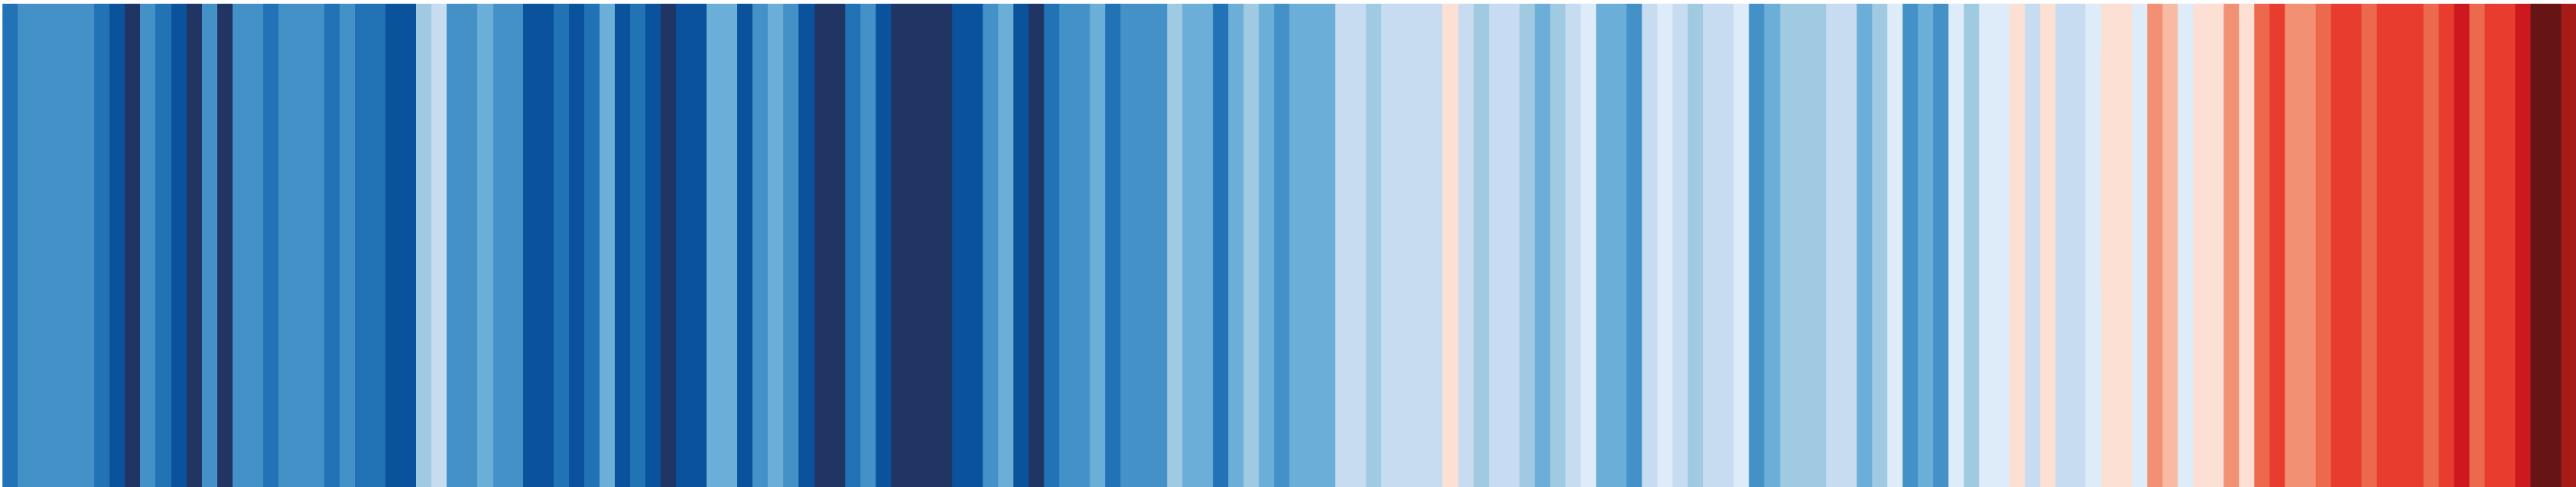
\includegraphics[width=\linewidth]{bilder/s4f-warming-stripes}
		\caption{Die Warming Stripes}
	\end{figure}
	\begin{itemize}
	\item[$\rightarrow$] Die langfristige Erwärmung und Häufung extremer Wetterereignisse bedeutet eine Veränderung des Klimas!
	\item[$\rightarrow$] Viele dieser Änderungen sind in Modellen der Klimaforscher relativ genau vorherzusagen.
	\item[$\rightarrow$] Das Ausmaß einiger Änderungen ist aufgrund der langfristigen Effekte nicht konkret vorherzusagen, aber die Tendenz ist klar.
	\item[$\rightarrow$] Der Klimawandel ist keine Naturkatastrophe, sondern menschengemacht. Wir können ihn in beide Richtungen beeinflussen. Je eher wir damit anfangen, desto leichter ist es.
	\end{itemize}

	\note{
	\begin{itemize}
		\item[] Wir haben nicht mehr wahnsinnig viel Zeit, jeder von uns sollte bei sich anfangen und etwas tun. Bereits kleine Dinge helfen: mehr mit dem Rad fahren, etwas weniger heizen, Reparieren oder gebraucht kaufen.
		\item[] Diese Vorlesung besuchen, mit den Dozenten und Zuhörern ins Gespräch kommen.
		\item[] Nach Projekt- und Abschlussarbeiten in diese Richtung Ausschau halten, oder einfach zu der Thematik anfragen.
		\item[] Sich mit anderen Austauschen und vernetzen.
		\item[$\rightarrow$] Übergang zu Engagement an der TU und darüber hinaus.
	\end{itemize}
	}
\end{frame}
